\section{3D Visualization Pipeline}
\label{sec.visualization_pipeline}

%This section reviews the viewing transform used by most popular graphics frameworks such as OpenGL. 

%Yet there is no standard way to specify the view, and there are a wide range of different viewing implementations currently in use.

%Closely tied in to viewing parameters is 3D interaction, and there are likewise a large number of different 3D interaction implementations often providing the same basic functionality. Users are forced to learn and use different pan, zoom, and spin techniques for each 3D program they use. As every 3D program has to reinvent this functionality,  OpenGL standard has emerged to supply the lack of standardization, the need of higher development and support efforts; as well as stifling the proliferation of user interface features like stereo. A standard viewing software toolkit, along with a standard motion toolkit, would benefit end users by delivering consistent and comprehensive 3D interaction across applications, and would benefit developers by reducing development time, software support, and customer support. All of the various interaction techniques can be provided to satisfy the varying requirements of the different types of 3D programs and the different levels of end user expertise.

The generation of 3D computer graphics is essentially a straightforward mapping of graphical items in a 3D volume, in a spatial domain $S$ in $\Re^3$, to a 2D image, in a spatial domain $S^{\prime}$ in $\Re^2$. Most viewing software use different transforms combined to deliver consistent and comprehensive 3D interactions: the model transform represents affine transformations, scale, translation and rotation, of each object in the 3D scene in the mapping $M_{model}: S_{model} \Rightarrow S_{scene}$; the view transform represents the individual transformations of every object in the 3D scene, representing the scene positioning for the viewer; which is the mapping $M_{view}: S_{view} \Rightarrow S_{scene}$; and the projection transform is the mapping $M_{proj}:S_{view} \Rightarrow S_{proj}$ that represents the perception of depth of the eye or camera. The final transform to 2D screen coordinates is $M_{screen}:S_{proj} \Rightarrow S^{\prime}_{screen}$. Note that in $M_{model}$ and $M_{view}$ the mapping is inverted to preserve the original spatial domain. Without loose of generality, all mappings can be defined as matrix transforms.

%The combination of the first and second transforms, view and model, is a single transform that translates and rotates the scene accordingly the viewer position, looking direction and view roll. This is an affine transform and the inverse  transform exists. Both transforms can be easily computed as a matrix in homogeneous coordinates. The latter transform projects the 3D scene into the output image. In most cases, the output image is a rectangular shape and the 3D view volume, called frustum, which is either a rectangular prism or a truncated pyramid for parallel and perspective views, respectively.


\subsection{OpenGL Pipeline}
\label{sec.opengl_pipeline}

In the OpenGL framework, the model and view transforms are combined in the \verb|GL_MODELVIEW| matrix. The 3D scene rendered by OpenGL must then be projected onto the computer screen using the \verb|GL_PROJECTION| matrix. In perspective projection, transforms a 3D point in a pyramid frustum in eye coordinates, truncated at the top, by the near plane $n$, and in the bottom, by the far plane $f$. The pyramid is bounded in $n$: in the horizontal by left and right coordinates, $l$ and $r$, and in the vertical by bottom and top coordinates, $b$ and $t$, respectively. The frustum is normalized in Normalized Device Coordinates (NDC), that is a mapping into a cube with the range of $x$-coordinate from $[l, r]$ to $[-1, 1]$, the y-coordinate from $[b, t]$ to $[-1, 1]$ and the $z$-coordinate from $[n, f]$ to $[-1, 1]$. The eye coordinates are defined in the left-handed coordinate system, but NDC uses the right-handed coordinate system. That is, the camera at the origin is looking along $-Z$ axis in eye space, but it is looking along $+Z$ axis in NDC. Since the OpenGL command glFrustum() accepts only positive values of near and far distances, they are negated during the construction of \verb|GL_PROJECTION| matrix.

\begin{figure}[h!]
\centering
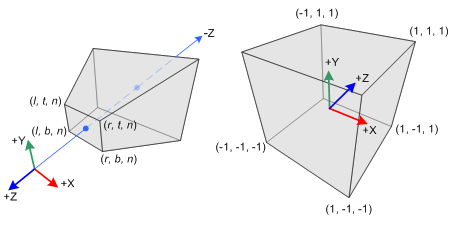
\includegraphics[width=0.9\linewidth,keepaspectratio=true]{figs/gl_projectionmatrix01.png}
\caption{Perspective Frustum and Normalized Device Coordinates (NDC)}
\label{fig.ndc}
\end{figure}

Part of the scene that is not going to be displayed, i.e., all vertex outside the frustum, is removed by frustum culling (clipping) and the edges of the polygon where clipping occurs are reconstructed. This is done transforming all vertex data from the eye coordinates, $(x_e, y_e, z_e)$, to the clip coordinate to clip coordinates $(x_c, y_c, z_c)$ in Equation~\ref{eq.clip}: 

\begin{equation}
\begin{aligned}
\begin{pmatrix} x_{c}\\y_{c}\\z_{c}\\w_{c} \end{pmatrix} &= 
M_{proj} \cdot \begin{pmatrix} x_{e}\\y_{e}\\z_{e}\\w_{e} \end{pmatrix}\\
%\begin{pmatrix} x_{ndc}\\y_{ndc}\\z_{ndc}\end{pmatrix} &=
%\begin{pmatrix} x_{c}/w_{c}\\y_{c}/w_{c}\\z_{c}/w_{c} \end{pmatrix}\\
\end{aligned}
\label{eq.clip}
\end{equation}

The clipping is performed in the clip coordinates by comparing with $w_c = -z_e$. If any clip coordinate is less than $-w_c$, or greater than $w_c$, then the vertex will be discarded. Then, those clip coordinates are also transformed to NDC by dividing the coordinates by the $w_c$ component in Equation~\ref{eq.ndc_coords}.
Bear in mind that both clipping and NDC transformations are integrated into \verb|GL_PROJECTION| matrix.

\begin{equation}
\begin{aligned}
\begin{pmatrix} x_{ndc}\\y_{ndc}\\z_{ndc}\end{pmatrix} &=
\begin{pmatrix} x_{c}/w_{c}\\y_{c}/w_{c}\\z_{c}/w_{c} \end{pmatrix}\\
\end{aligned}
\label{eq.ndc_coords}
\end{equation}

Then, a 3D point in eye space is projected onto the near plane. The following diagrams show how a point $(x_e, y_e, z_e)$ in eye space is projected to $(x_p, y_p, z_p)$ on the near plane.

\begin{figure}[h!]
\centering
\begin{tabular}{cc}
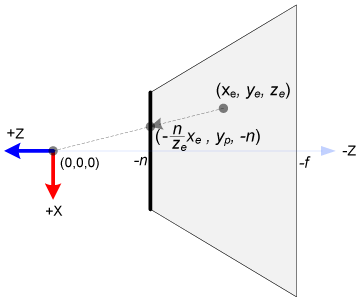
\includegraphics[width=0.45\linewidth,keepaspectratio=true]{figs/gl_projectionmatrix03.png}
&
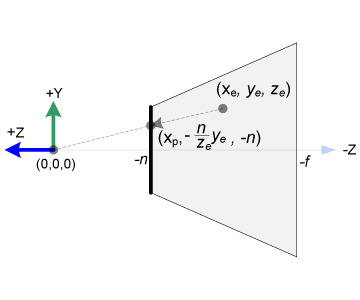
\includegraphics[width=0.45\linewidth,keepaspectratio=true]{figs/gl_projectionmatrix04.png}
\\
(a) Top View of Frustum
&
(b) Side View of Frustum
\end{tabular}
\label{fig.frustum}
\caption{Views of the frustum.}
\end{figure}

%From the top view of the frustum, the $x$-coordinate of eye space, $x_e$ is mapped to $x_p$, which is calculated by using the ratio of similar triangles;

%\begin{equation}
%\begin{aligned}
%\begin{split}
%\frac{x_p}{x_e}&=\frac{-n}{z_e}\\
%x_p&=\frac{-n \cdot x_e}{z_e}\\
%   &=\frac{n \cdot x_e}{-z_e}
%\end{split}
%\end{aligned}
%\label{eq.xp}
%\end{equation}

%From the side view of the frustum, $y_p$ is also calculated in a similar way; 

%\begin{equation}
%\begin{aligned}
%\begin{split}
%\frac{y_p}{y_e}&=\frac{-n}{z_e}\\
%y_p&=\frac{-n \cdot y_e}{z_e}\\
%   &=\frac{n \cdot y_e}{-z_e}
%\end{split}
%\end{aligned}
%\label{eq.yp}
%\end{equation}

Note that both $x_p$ and $y_p$ depend on $z_e$; they are inversely proportional to $-z_e$. In other words, they are both divided by $-z_e$. It is a very first clue to construct \verb|GL_PROJECTION| matrix. Therefore, the $w$-component of the clip coordinates is set as $-z_e$. And, the 4th row of \verb|GL_PROJECTION| matrix becomes $(0, 0, -1, 0)$: 

\begin{equation}
\begin{aligned}
\begin{split}
\begin{pmatrix} x_{c}\\y_{c}\\z_{c}\\w_{c} \end{pmatrix} &= 
\begin{pmatrix} 
\cdot & \cdot & \cdot & \cdot \\
\cdot & \cdot & \cdot & \cdot \\
\cdot & \cdot & \cdot & \cdot \\
0 & 0 & -1 & 0 \\
\end{pmatrix} &=
\begin{pmatrix} x_{e}\\y_{e}\\z_{e}\\w_{e} \end{pmatrix}
\end{split}
\end{aligned}
\label{eq.rows}
\end{equation}

%\begin{figure}[h!]
%\centering
%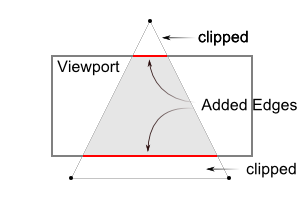
\includegraphics[width=0.9\linewidth,keepaspectratio=true]{figs/gl_frustumclip.png}
%\caption{A triangle clipped by frustum}
%\label{fig.clipping}
%\end{figure}

When all other entries in Equation~\ref{eq.rows} are obtained~\cite{schreiner2004}, the complete projection matrix is: 

\begin{equation}
\begin{aligned}
M_{proj} &= 
\begin{pmatrix} 
\frac{2n}{r-l} & 0 & \frac{r+l}{r-l} & 0 \\
0 & \frac{2n}{t-b} & \frac{t+b}{t-b} & 0 \\
0 & 0 & -\frac{f+n}{f-n} & -\frac{2fn}{f-n} \\
0 & 0 & -1 & 0 \\
\end{pmatrix} \\
\end{aligned}
\label{eq.projection_matrix}
\end{equation}




\subsection{Stereo Visualization}
\label{sec.stereo_visualization}

Let the distance of the eye to the screen, $d_{s}$, and the intra-ocular separation, $d_{io}$. Stereo view is enabled by translating the view off-center to the left by $d_{eye} = -d_{io}/2$,  and to the right by $d_{eye} = d_{io}/2$, as shown in Figure~\ref{fig.stereo_views}a. The view is split for left and right eyes using $M_{eye}$ in Equation~\ref{eq.stereo_view_matrix} combined with $M_{view}$.

\begin{equation}
\begin{aligned}
M_{eye} &= 
\begin{pmatrix} 
1 & 0 & 0 & d_{eye}\\
0 & 1 & 0 & 0\\
0 & 0 & 1 & 0\\
0 & 0 & 0 & 1\\
\end{pmatrix}
\end{aligned}
\label{eq.stereo_view_matrix}
\end{equation}

\begin{figure}[!hb]
\centering
\begin{tabular}{cc}
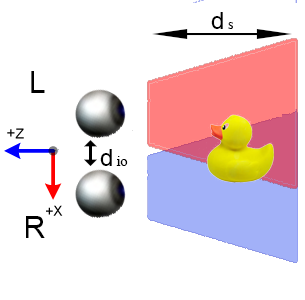
\includegraphics[width=0.35\linewidth,keepaspectratio=true]{figs/stereo_offset.png}
&
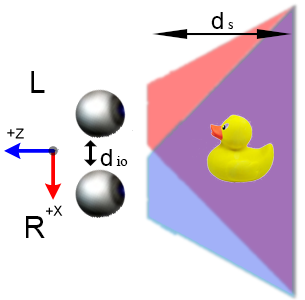
\includegraphics[width=0.35\linewidth,keepaspectratio=true]{figs/stereo_shear.png}
\\
(a)&(b)
\end{tabular}
\caption{Stereo views.}
\label{fig.stereo_views}
\end{figure}

Regarding the stereo technique to display the left and right views, adjustments in the horizontal, $s_x$, or vertical, $s_y$, scales are applied after the stereo view. In case of the modulation of the right and left views along time, there is no split and the view is fully displayed using  $s_x = s_y = 1$. In case of stereo split of the screen, each left and right views are scaled to half by $s_x = 2$, in case of vertical split, or by $s_y = 2$, in case of horizontal split. Both splits can be used to create the intertwined lines of right and left eye polarization.  

The convergence point is moved from $z=-\infty$ towards $+z$ by the shearing, as shown in Figure~\ref{fig.stereo_views}b, of the left and right projection frustum by $sh_z = d_{eye}/d_{s}$. The final stereo projection matrix, $M_{stereo}$, is a matrix scaled by $s_x$ and $s_y$, and sheared $sh_z$ in Equation~\ref{eq.stereo_proj_matrix}. The stereo pipeline is the sequence of transformations: $M_{stereo} \times M_{proj} \times M_{eye} \times M_{view}$.

\begin{equation}
\begin{aligned}
M_{stereo} &= 
\begin{pmatrix} 
s_x & 0 & 0 & 0\\
0 & s_y & 0 & 0\\
0 & 0   & 1 & 0\\
0 & 0   & 0 & 1\\
\end{pmatrix}
\begin{pmatrix} 
1 & 0 & sh_z & 0\\
0 & 1 & 0 & 0\\
0 & 0 & 1 & 0\\
0 & 0 & 0 & 1\\
\end{pmatrix}
\end{aligned}
\label{eq.stereo_proj_matrix}
\end{equation}

 